\documentclass{beamer}
\usepackage{graphicx}  % Required for including images
\usepackage{amsmath}
\usepackage{url}
\usepackage{upquote}

\title{Intro to R Packages}
\author{Eric Fox}
\date{\today}

\begin{document}

\frame{\titlepage}

%--------------------------------------------------------------------
\begin{frame}
Main reference is Hadley Wickam's book ``R Packages", which is available for free online:\\
\vspace{3ex}
\url{http://r-pkgs.had.co.nz/}\\
\vspace{3ex}
\centering
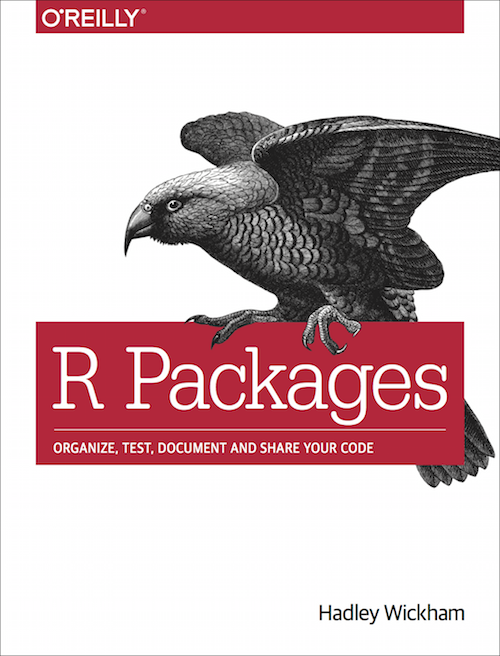
\includegraphics[width=0.25\textwidth]{figure/cover.png}
\end{frame}

%--------------------------------------------------------------------
\begin{frame}{Motivation}
Why learn how to create R packages in RStudio:
\vspace{1ex}
\begin{itemize}
\item Easily share code and collaborate with others.
\vspace{1ex}
\item Bundle R functions, data sets, and documentation together.
\vspace{1ex}
\item Provides a consistent template and set of tools for organizing large research projects. 
\end{itemize}
\end{frame}

%--------------------------------------------------------------------
\begin{frame}[fragile]{Getting started}
First, make sure you have the following packages installed:
\begin{verbatim}
install.packages(c("devtools", "roxygen2", "knitr"))
\end{verbatim}
\end{frame}

%--------------------------------------------------------------------
\begin{frame}{Getting started}
The process of setting up an R package in RStudio is documented here:\\
\vspace{3ex}
\url{http://r-pkgs.had.co.nz/package.html}\\
\vspace{3ex}
If you are using a government computer make sure you use the \texttt{C:/} drive as the directory for your package.  R packages will not work on the network.
\end{frame}

%--------------------------------------------------------------------
\begin{frame}{Components of an R package}
\begin{itemize}
\item \textbf{R functions}:  all R functions are placed in the \texttt{R/} directory.
\vspace{1ex}
\item \textbf{Documentation}: write documentation for your functions so that others (and future you!) can easily use your package.  Documentation exists in the \texttt{man/} directory, but can be included with your R function code using \texttt{roxygen2}.
\vspace{1ex}
\item \textbf{Data}: place data sets in the \texttt{data/} directory for easy access.
\vspace{1ex}
\item \textbf{Installed files}: \texttt{inst/} is the `anything goes' directory; you are free to put anything you like in this folder (e.g., R markdown reports, manuscript drafts, etc.).
\end{itemize}
\end{frame}

%--------------------------------------------------------------------
%\begin{frame}{Components of a R package}
%The following files are automatically generated when you create a package in RStudio:
%\vspace{1ex}
%\begin{itemize}
%\item \texttt{Description} file: allows you to add metadata to your package.
%\vspace{1ex}
%\item \texttt{Namespace} file: provides ``spaces" for ``names"; you may have already encountered the concept of namespaces when using the \texttt{::} operator in R.
%\end{itemize}
%\end{frame}

%--------------------------------------------------------------------
\begin{frame}{Components of an R package}
The automatically generated \texttt{Description} and \texttt{Namespace} files are sufficient for most purposes.  If you would like to learn more about these topics I suggest reading:\\
\vspace{3ex}
\url{http://r-pkgs.had.co.nz/namespace.html}\\
\url{http://r-pkgs.had.co.nz/description.html}\\
\vspace{3ex}
Although, understanding these components is not necessary to start creating your own R packages.
\end{frame}

%--------------------------------------------------------------------
\begin{frame}{Components of an R package}
Default directory structure for package created in RStudio.\\
\vspace{3ex}
\centering
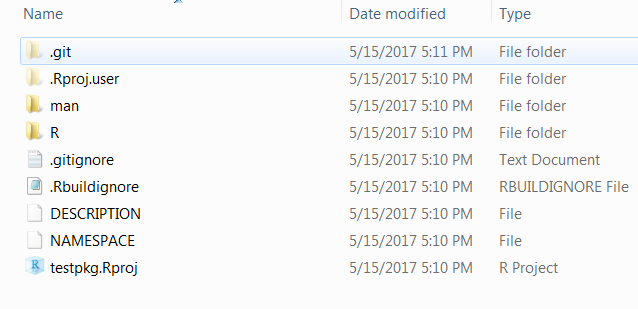
\includegraphics[width=0.7\textwidth]{figure/pkg1.png}
\end{frame}

%--------------------------------------------------------------------
\begin{frame}{Components of an R package}
I usually add \texttt{data/} and \texttt{inst/} folders since these are useful components of a package, especially for research projects.\\
\vspace{3ex}
\centering
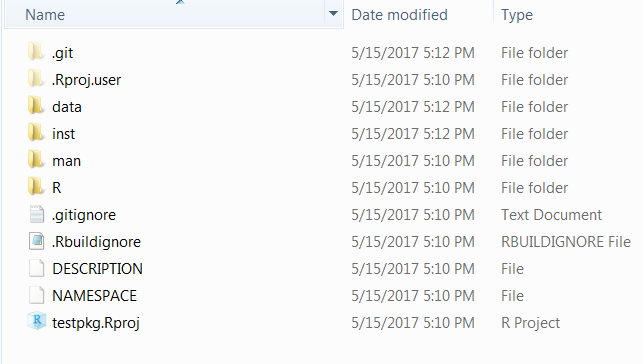
\includegraphics[width=0.7\textwidth]{figure/pkg2.png}
\end{frame}

%--------------------------------------------------------------------
\begin{frame}[fragile]{Example 1: R function and documentation}
\begin{verbatim}
#' Add together two numbers.
#'
#' @param x A number.
#' @param y A number.
#' @return The sum of \code{x} and \code{y}.
#'
#' @examples
#' add(1, 1)
#' add(10, 1)
#'
#' @export
add <- function(x, y) {
  x + y
}
\end{verbatim}
\end{frame}

%--------------------------------------------------------------------
\begin{frame}[fragile]{Loading R functions}
To load all R functions in your package use the following command:
\begin{verbatim}
devtools::load_all(".")
\end{verbatim}
Or use the shortcut \emph{Ctl + Shift + L}\\
\vspace{2ex}
Each time your change or debug your R functions run this command.\\
\end{frame}

%--------------------------------------------------------------------
\begin{frame}[fragile]{Processing documentation}
Run the following command so that roxygen documentation can be previewed in the help pane:\\
\begin{verbatim}
devtools::document()
\end{verbatim}
Technically, this command converts the roxygen comments into R documentation files (.Rd) which are placed in the \texttt{man/} directory.\\
\vspace{2ex}
Each time you edit your function's roxygen documentation run this command and then preview documentation in the help menu.\\
% show example with help menu
\end{frame}

%--------------------------------------------------------------------
\begin{frame}{Example 1: R function and documentation}
\centering
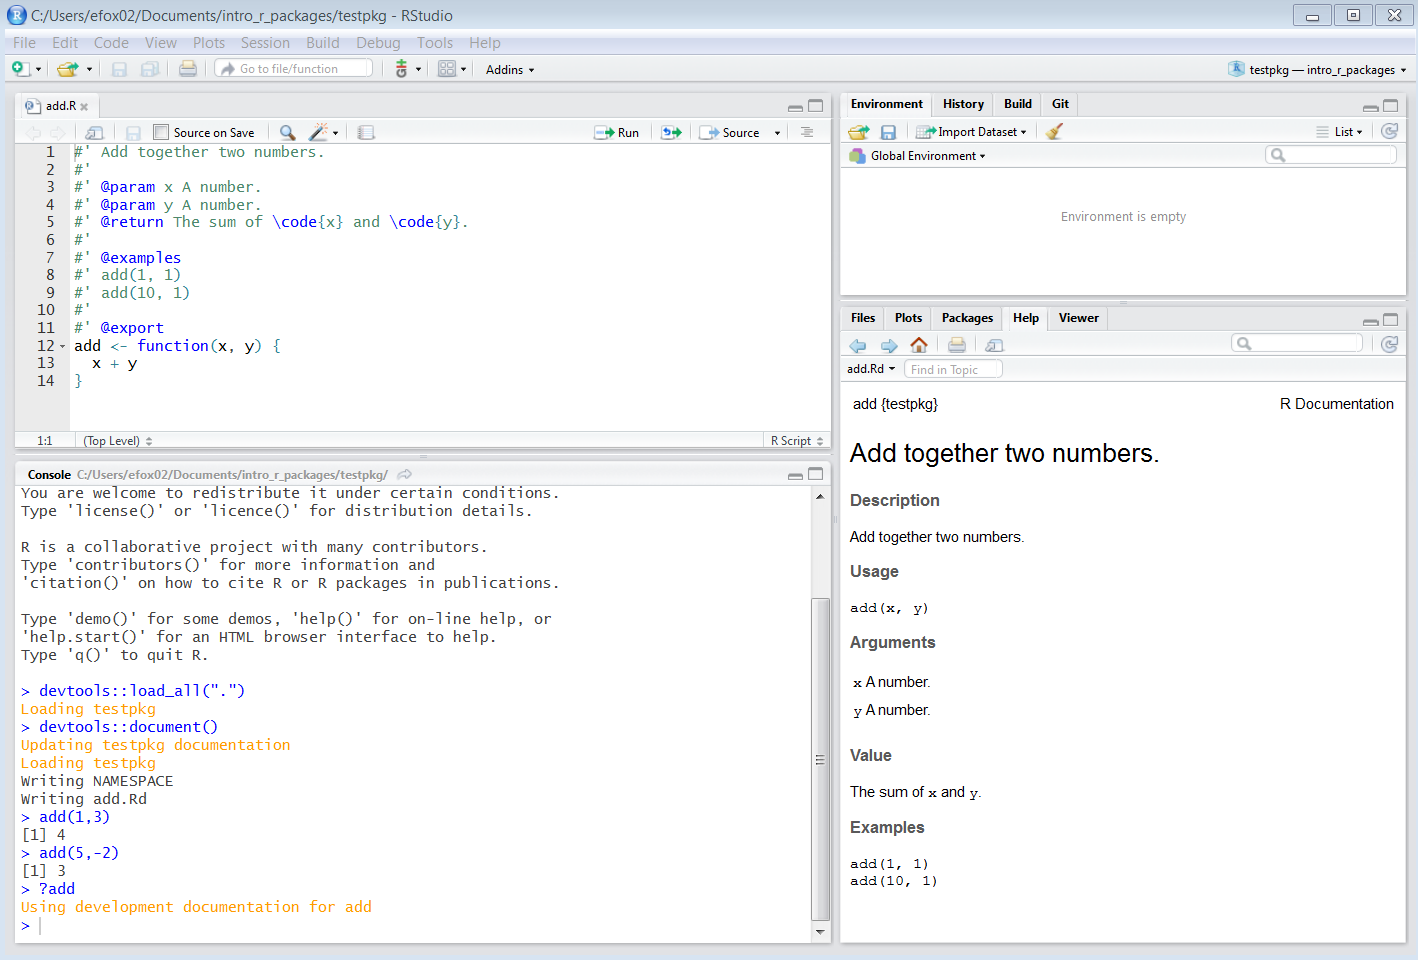
\includegraphics[width=0.9\textwidth]{figure/Ex1.png}
\end{frame}

%--------------------------------------------------------------------
\begin{frame}{Build a R packages}
\begin{itemize}
\item Click `Build \& Reload' in the RStudio Build pane to build, install, and then reload your R package.
\item This will enable you to use the \texttt{library()} function to load your package.
\item Building a package can be slow, so if you are in the development stage I recommend using the \texttt{devtools} functions (\texttt{load\_all()} and \texttt{document()}) instead.
\end{itemize}
\centering
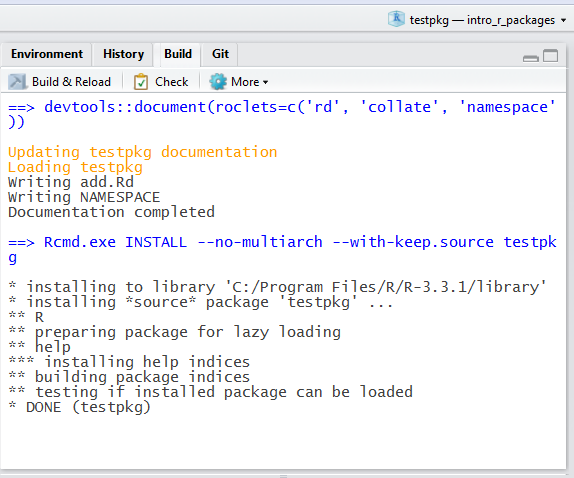
\includegraphics[width=0.3\textwidth]{figure/buildpane.png}
\end{frame}

%--------------------------------------------------------------------
\begin{frame}{Data/}
\begin{itemize}
\item Data sets placed in the \texttt{data/} directory will become readily available when you load your package (e.g., using \texttt{load\_all()} or a manually building and using \texttt{library()}).
\vspace{1ex}
\item Save data sets in \texttt{data/} as \texttt{.RData} files. 
\vspace{1ex}
\item You can also document data sets using roxygen style comments.  See `Documenting datasets' section of \url{http://r-pkgs.had.co.nz/data.html} for an example.
\end{itemize}
\end{frame}

%--------------------------------------------------------------------
\begin{frame}{Inst/}
\begin{itemize}
\item You can place anything you like in the \texttt{inst/} directory.
\vspace{1ex}
\item Some examples:
\begin{itemize}
\item R markdown reports,
\item manuscript drafts,
\item R scripts, etc.
\end{itemize}
\vspace{1ex}
\item Only exception is don't use an existing package directory name (e.g., avoid \texttt{inst/R} or \texttt{inst/data}).
\end{itemize}
\end{frame}

%--------------------------------------------------------------------
\begin{frame}{Example 2}
Write an R function and documentation for computing the root-mean-square error defined as:
\begin{align*}
RMSE = \sqrt{\frac{1}{n}\sum_{i=1}^n (y_i - \hat{y}_i)^2}
\end{align*} 
where $y_i$ is an observed value and $\hat{y}_i$ is a predicted value (e.g., from a linear model).
\end{frame}

%--------------------------------------------------------------------
\begin{frame}[fragile]{Example 2}
\small
\begin{verbatim}
#' RMSE
#' 
#' A function that computes the root-mean-square error (RMSE).
#' 
#' @param y Numeric vector of observed values.
#' @param yhat Numeric vector of predictions.
#' @return RMSE
#'   
#' @export
compute_rmse <- function(y, yhat) {
  n <- length(y)
  sqrt((1 / n) * sum((y - yhat)^2))
}
\end{verbatim}
\end{frame}

\end{document}




